\documentclass[lettersize,journal]{IEEEtran}
\usepackage{amsmath,amsfonts}
\usepackage{algorithmic}
\usepackage{array}
\usepackage[caption=false,font=normalsize,labelfont=sf,textfont=sf]{subfig}
\usepackage{textcomp}
\usepackage{stfloats}
\usepackage{placeins}
\usepackage{url}
\usepackage{verbatim}
\usepackage{graphicx}
\hyphenation{op-tical net-works semi-conduc-tor IEEE-Xplore}
\def\BibTeX{{\rm B\kern-.05em{\sc i\kern-.025em b}\kern-.08em
    T\kern-.1667em\lower.7ex\hbox{E}\kern-.125emX}}
\usepackage{balance}
\begin{document}
\title{OrbitGraph: Graph-Centric Software Defined Routing for LEO Satellite Constellations}

\author{\IEEEauthorblockN{
    Gustavo Pantuza\IEEEauthorrefmark{1},
    Luiz F. M. Vieira\IEEEauthorrefmark{1},
    Marcos A. M. Vieira\IEEEauthorrefmark{1}
}\\
\IEEEauthorblockA{
    \IEEEauthorrefmark{1}Department of Computer Science, Universidade Federal de Minas Gerais - Brazil
}


\thanks{Manuscript created on June, 2026; This work was developed by the LeCom laboratory from the Department of Computer Science of Federal University of Minas Gerais (UFMG).}
}

\markboth{IEEE Transactions on Computers,~Special Issue on Graph-Centric Computing}%
{Pantuza \MakeLowercase{\textit{et al.}}: OrbitGraph: Graph-Centric Software-Defined Routing for LEO Constellations}

\maketitle


% Abstract and keywords for the IEEE TC Graph-Centric Computing special issue.

% Title: OrbitGraph: Graph-Centric Software Defined Routing for LEO Satellite Constellations

\begin{abstract}
Low Earth orbit constellations form \emph{dynamic graphs}: links and weights change
as satellites move and ground-satellite contacts hand over.
Distributed OSPF must reconverge after each topology change, which can interrupt
end-to-end forwarding for multiple seconds.
We propose OrbitGraph, a graph-centric software-defined routing scheme that
recomputes shortest paths centrally and pushes only changed kernel routes
\emph{before} the old ground-satellite link is torn down.
Using container-based emulation from 27 to 100 satellites (including 2 ground stations), 
we measure control-plane cost and data-plane availability with a continuous outage 
probe aligned to routing events.
On coverage-preserving handovers, OrbitGraph yields 0\,ms data-plane outage and
0\% packet loss, while OSPF incurs multi-second black holes (up to ${\sim}15$\,s).
OrbitGraph pushes 524 kernel routes at the largest constellation versus 10\,504
at full initialization, and Dijkstra recomputation remains in the millisecond range.
When the constellation is too sparse to keep a ground station in view, a coverage
gap severs the ground-to-ground path for both protocols, bounding where
control-plane update ordering helps.
\end{abstract}

\begin{IEEEkeywords}
Dynamic graphs,
LEO satellite networks,
software-defined networking,
topology handover,
incremental routing,
network emulation,
graph-centric systems,
data-plane availability,
routing scalability
\end{IEEEkeywords}

% Introduction (Kurose 5-paragraph structure).

\section{Introduction}
\label{sec:intro}

Low Earth orbit (LEO) mega-constellations have become a mainstream component of
the global Internet: hundreds to thousands of satellites at a few hundred
kilometers of altitude now deliver low-latency broadband to regions that
terrestrial infrastructure cannot economically reach~\cite{smallsats2020,
handley:ground-relays:2019}.
Their low altitude yields round-trip times competitive with, and sometimes
better than, long-haul fiber, which has driven intense study of constellation
design and performance at scale~\cite{kassing2020exploring,lai2020starperf}.
As these systems grow to thousands of nodes carrying production traffic, the
network layer faces a defining challenge: it must keep packets flowing while the
physical topology is in perpetual, rapid motion.

Because satellites orbit continuously, a LEO network is most naturally described
as a \emph{time-varying graph} in which inter-satellite and ground--satellite
links (GSLs) appear and disappear on a schedule dictated by orbital
mechanics~\cite{seong:topological-design:1995,kassing2020exploring}.
A ground station must therefore hand its uplink from a setting satellite to a
rising one at recurring, predictable instants, a GSL \emph{handover}.
Distributed link-state routing such as open shortest path first
(OSPF)~\cite{sidhu:ospf:1993}, the de facto baseline in container-based LEO
emulators~\cite{lai2023starrynet}, learns each mutation reactively through
hello timeouts and link-state flooding, and reconverges only \emph{after} the
link change has completed.
During that interval, traffic is forwarded along stale or missing next-hops and
is silently black-holed.
This raises the central question of this paper: since handover times are known
in advance from orbital prediction, can routing exploit that knowledge to keep
the data plane continuously connected across topology changes?

In this paper we present OrbitGraph, a graph-centric, software-defined routing
scheme for LEO constellations.
OrbitGraph models each orbital snapshot as a delay-weighted graph $G_t$, computes
all-pairs shortest paths centrally with Dijkstra's algorithm, and programs the
kernel forwarding information base (FIB) of each node by pushing only the routes
that changed since the previous snapshot.
At a handover, the controller installs the post-handover FIB \emph{before} the
old GSL is torn down, turning orbital predictability into make-before-break
forwarding at the topology level.
We implement OrbitGraph~\cite{online:orbitgraph:2025} on the StarryNet emulator~\cite{lai2023starrynet}, which
runs real TCP/IP stacks and an OSPF control plane in containers, and evaluate it
against that distributed baseline on Walker constellations from 27 to 102 nodes
using a continuous outage probe aligned to routing events.
Our contributions are fourfold: a graph-centric software-defined networking
(SDN) control model that unifies initialization, delay refresh, link failure,
and GSL handover as shortest-path computations over a sequence of snapshots
$G_t$; an incremental, make-before-break FIB install that programs only changed
next-hops, reducing handover updates by roughly two orders of magnitude relative
to a full-table push; a proactive handover mechanism that commits the new
forwarding state while both contacts briefly coexist; and an empirical study
showing 0\,ms data-plane outage on coverage-preserving GSL handovers where OSPF
incurs multi-second black holes, alongside millisecond-range shortest-path
recomputation, together with a characterization of the boundaries of the
approach: a satellite coverage gap that severs the path for both protocols, and
unplanned bulk failure where centralized install does not yet outperform
distributed reconvergence.

OrbitGraph differs from prior LEO routing along a single axis: \emph{what}
forwarding state to install and \emph{when} relative to link lifetime.
Snapshot and offline schemes precompute per-state tables and load them on
board~\cite{seong:topological-design:1995}; distributed protocols optimize hop
count or convergence speed without a global view~\cite{gregory:satellite-routing:2022,
pam:opspf:2019}; and satellite SDN research has largely targeted controller
\emph{placement} rather than route computation~\cite{papa:sdn-cpp:2018,
guo:spda:2022}.
To our knowledge, none of these install real kernel forwarding state on emulated
satellite nodes and measure end-to-end availability through handover under
proactive update ordering; Section~\ref{sec:related} compares these lines in
detail.

The remainder of this paper reviews software-defined and graph-centric
networking principles, situates OrbitGraph among prior LEO routing work,
describes the StarryNet emulation platform and OrbitGraph design, reports the
scaling methodology and results, discusses limitations, and concludes.

\input{03-sdn-background}
% Related work section for OrbitGraph paper.

\section{Related Work}
\label{sec:related}

Prior LEO routing work spans snapshot and centralized schemes, distributed
protocols, satellite SDN management, evaluation platforms, and broader
networking literature, which we contrast with OrbitGraph's graph-centric,
proactive SDN forwarding model.

\subsection{Centralized and snapshot routing}

LEO constellations have been modeled as finite-state automata whose states are
recurring visibility configurations, with inter-satellite link assignment and
multi-commodity routing optimized offline per
state~\cite{seong:topological-design:1995}.
That strategy avoids transient instability but relies on offline computation for
a small constellation (12 satellites) and ignores online failure recovery.
OrbitGraph shares the snapshot view but computes shortest paths online and
installs kernel routes through an SDN controller rather than storing per-state
tables on satellites.

Wide-area routing in mega-constellations with and without inter-satellite links
(ISLs) has been studied, emphasizing ground-relay paths when ISLs are absent and
hierarchical, tile-based updates when centralized Dijkstra over thousands of
relays is too slow~\cite{handley:ground-relays:2019}.
Unlike OrbitGraph, that line targets constellation design and relay selection,
not in-container forwarding during live GSL handover, and does not compare
against a distributed interior gateway protocol (IGP) baseline.

\subsection{Distributed LEO routing protocols}

DisCoRoute is a distributed on-demand algorithm for Walker-Delta
mega-constellations that derives a closed-form minimum hop count between orbital
identifiers and selects the next hop in constant time, reporting large speedups
at up to 32\,000 satellites~\cite{gregory:satellite-routing:2022}.
It optimizes hop count on a fixed +Grid ISL pattern and does not model link
failures or convergence delay.
OrbitGraph instead centralizes shortest-path computation on delay-weighted
graphs and measures end-to-end outage during handover.

Orbit-predictive shortest path first (OPSPF) keeps OSPF-style hello and
link-state machinery but uses orbit prediction so regular motion generates no
protocol traffic, with only failures triggering updates~\cite{pam:opspf:2019}.
Evaluated on 48 satellites, it reduces convergence time over vanilla OSPF.
OrbitGraph removes distributed flooding entirely, recomputing $G_t$ from
ephemeris and programming routes directly to target zero handover outage through
proactive install ordering.

Our OSPF baseline, BIRD on StarryNet~\cite{lai2023starrynet}, represents the
reactive link-state approach from early protocol studies~\cite{sidhu:ospf:1993}
and widely used in LEO evaluations~\cite{manzanareslopez2025comprehensive}.
It reconverges only after full topology mutation, which
Section~\ref{sec:analysis} shows can black-hole traffic for several seconds at
GSL handover, the behavior OrbitGraph eliminates.

Terrestrial ad hoc routing, such as ad hoc on-demand distance vector
(AODV)~\cite{perkins:aodv:1999} and greedy perimeter stateless routing
(GPSR)~\cite{karp:gpsr:2000}, targets unpredictable mobility without orbital
models, and ns-3-leo reports that such mobile ad hoc network (MANET) protocols
perform poorly in dynamic satellite scenarios~\cite{ns3leo2022}.
OrbitGraph exploits the opposite assumption: topology is predictable from
SGP4-based delay matrices, so a centralized graph controller is feasible.

A recent robustness study shows that inter-satellite link failures from
environmental and load factors degrade static routing far more than dynamic or
distributed approaches~\cite{yang:leo-routing-resilience:2025}, motivating the
failure-mode analysis we report for OrbitGraph under satellite damage.

\subsection{SDN and graph-based network management}

The SDN paradigm separates control and data planes and enables programmatic
forwarding through interfaces such as OpenFlow~\cite{10.1145/1355734.1355746}.
Representing an SDN domain as a graph gives controllers a unified structure for
topology-aware management and shortest-path algorithms~\cite{7014202}, which
OrbitGraph applies to time-varying LEO snapshots rather than terrestrial
OpenFlow switches.

Satellite-specific SDN research has focused on controller placement, not
data-plane route computation.
Dynamic placement on an Iridium-class 66-satellite constellation has been cast
as an integer linear program minimizing average flow setup
time~\cite{papa:sdn-cpp:2018}, while static placement adapts
switch-to-controller bindings to topology snapshots on Iridium and Celestri
models~\cite{guo:spda:2022}.
Both optimize control placement and treat forwarding as a black box, whereas
OrbitGraph addresses what routes to install and when relative to link lifetime,
evaluating data-plane availability during handover rather than switch-controller
latency.

Centralized traffic engineering has also been applied to satellite backbones,
where a controller computes low-latency routes across a time-varying topology to
meet flow-level objectives~\cite{wu:sate-satellite-te:2025}.
That work optimizes path selection and load balancing at the traffic-matrix
level, whereas OrbitGraph targets per-handover forwarding continuity measured as
data-plane outage on emulated nodes.

\subsection{Simulation and emulation platforms}

The ns-3-leo module~\cite{ns3leo2022} adds orbital mobility, ISLs, and MANET
routing to discrete-event simulation, highlighting limitations of terrestrial
protocols in space.
A dedicated LEO simulator provides configurable +Grid and sparse ISL topologies
with 3D visualization~\cite{kempton:network-simulator:2021}, and the underlying
SILLEO-SCNS tool~\cite{kempton2020silleo,online:silleo:2025} focuses on topology
generation rather than packet-level stacks.
Simplified OMNeT++~5 scenarios support rapid
prototyping~\cite{dewangan:simple-omnet:2017}.
These platforms either lack real protocol stacks or use distributed routing
without centralized proactive install.

Packet-level ns-3 frameworks are surveyed
comprehensively~\cite{manzanareslopez2025comprehensive}.
Hypatia~\cite{kassing2020exploring} runs ns-3 with static Floyd--Warshall
routing, StarPerf~\cite{lai2020starperf} profiles area-to-area performance, and
LEOPath~\cite{leopath2024} targets routing-algorithm comparison without
end-to-end kernel forwarding.
StarryNet~\cite{lai2023starrynet} emulates real TCP/IP and OSPF in containers
and is our evaluation harness, which OrbitGraph extends with a centralized
controller, incremental kernel route install, and proactive handover
(Section~\ref{sec:simulation}).
A recent review of LEO/NTN routing spanning classical, learning-based, and
quantum methods finds the evidence base predominantly simulation-driven, with
limited testbed or emulation support and often simplified control-plane
realism~\cite{mattar:leo-ntn-routing-perspectives:2026}, a gap OrbitGraph
addresses by evaluating real kernel forwarding under a centralized controller in
container emulation.

\subsection{Broader LEO networking literature}

Growing interest in large LEO and swarm systems motivates global, low-latency
connectivity~\cite{smallsats2020,asri2024swarm,farrag:swarm-survey:2021}.
Swarm intelligence frameworks~\cite{chen2022swarm} and formation control
studies~\cite{fangchen2022pdg} address mission-layer coordination, not IP
handover, and machine-learning routing is surveyed with emphasis on model design
and deployment~\cite{zhu:ml-routing-survey:2025}, with recent work applying deep
graph reinforcement learning to routing on large-scale LEO
topologies~\cite{huang:graph-rl-leo-routing:2026}.
An earlier environment for distributed routing analysis in LEO
swarms~\cite{online:silleo-routing:2025} compared conventional protocols without
a centralized proactive strategy.
OrbitGraph instead uses explicit graph snapshots and Dijkstra shortest paths
with deterministic SDN install ordering, quantifying data-plane outage on the
same class of emulated constellations for reproducible comparison with OSPF.

\subsection{Positioning of OrbitGraph}

Table~\ref{tab:related-positioning} summarizes how OrbitGraph relates to the
closest prior lines.
Prior snapshot and centralized schemes optimize offline tables or relay
placement, distributed protocols optimize hop count or OSPF convergence, and
satellite SDN papers optimize controller placement.
OrbitGraph combines online graph snapshots, centralized delay-weighted shortest
paths, incremental dataplane deltas, and proactive GSL handover in one emulated
system with measured end-to-end outage, a combination absent from these works.

\begin{table}[!h]
  \centering
  \caption{OrbitGraph vs.\ representative related work (selected dimensions).}
  \label{tab:related-positioning}
  \renewcommand{\arraystretch}{1.1}
  \footnotesize
  \begin{tabular}{@{}lcccc@{}}
    \hline
    Work & Central & Real FIB & Proactive HO & Outage eval. \\
    \hline
    Snapshot routing~\cite{seong:topological-design:1995} & Yes & No  & offline & No \\
    DisCoRoute~\cite{gregory:satellite-routing:2022} & No  & No  & No      & No \\
    OPSPF~\cite{pam:opspf:2019} & No  & Yes & partial & partial \\
    SDN placement~\cite{papa:sdn-cpp:2018,guo:spda:2022} & Yes & No  & No      & No \\
    StarryNet OSPF~\cite{lai2023starrynet} & No  & Yes & No      & Yes \\
    OrbitGraph (this work) & Yes & Yes & Yes     & Yes \\
    \hline
  \end{tabular}
  \\[0.4em]
  \footnotesize
  HO: handover. Real FIB: kernel or protocol forwarding on emulated nodes.
\end{table}

% Simulation environment section for OrbitGraph paper.

\section{Simulation Environment}
\label{sec:simulation}

Evaluating routing under realistic LEO dynamics requires a platform that can
evolve topology and link delays as satellites move, exercise real intra-domain
routing or an equivalent control-plane install path, and exchange packets
end-to-end with measurable latency and loss.
We surveyed representative LEO simulators and emulators following a recent
ns-3-based framework review~\cite{manzanareslopez2025comprehensive}.
Table~\ref{tab:simulators} summarizes the alternatives we considered; we adopt
StarryNet~\cite{lai2023starrynet} for the experiments in this paper.

\begin{table}[!h]
  \centering
  \caption{LEO simulation platforms considered for OrbitGraph evaluation.}
  \label{tab:simulators}
  \renewcommand{\arraystretch}{1.15}
  \begin{tabular}{@{}lccc@{}}
    \hline
    Platform & Packet-level & Real routing & Live topology \\
    \hline
    SILLEO-SCNS~\cite{kempton2020silleo}      & No  & No  & Yes \\
    Hypatia~\cite{kassing2020exploring}       & Yes & No  & Yes \\
    LEOPath~\cite{leopath2024}                & No  & No  & Yes \\
    StarPerf~\cite{lai2020starperf}           & No  & No  & Yes \\
    StarryNet~\cite{lai2023starrynet}         & Yes & Yes & Yes \\
    \hline
  \end{tabular}
  \\[0.5em]
  \footnotesize
  Real routing: distributed protocols (e.g., OSPF) or kernel FIB install on
  emulated nodes, not precomputed abstract paths alone.
\end{table}

\subsection{Candidate platforms and selection rationale}

SILLEO-SCNS (Simulator for Large LEO Satellite Communication
Networks)~\cite{kempton2020silleo} focuses on constellation generation, orbital
motion, and inter-satellite connectivity modeling.
It offers strong topology visualization and scales well for studying link
geometry.
However, it does not perform packet-level network simulation: there is no
end-to-end traffic exchange through a real or emulated protocol stack, so it
cannot directly measure round-trip time (RTT), jitter, or sustained data-plane
outage around routing events, metrics central to our OrbitGraph evaluation.

Hypatia~\cite{kassing2020exploring} integrates precomputed orbital state with
the ns-3 discrete-event simulator and supports packet-level experiments at LEO
scale.
Its routing layer, however, relies on precomputed shortest paths (e.g.,
Floyd--Warshall) rather than running distributed protocols such as OSPF or an
operator-style centralized install.
That design is well suited to capacity and latency characterization but does
not let us compare distributed reconvergence against proactive SDN-style
updates on identical emulated topologies.
In addition, full ns-3 campaign runtimes reported in the literature are
substantially longer than container emulation for comparable scenario
complexity.

LEOPath~\cite{leopath2024} is a Python framework for analyzing and comparing
routing algorithms over time-varying LEO graphs.
It is more extensible than static shortest-path pipelines and targets routing
research directly.
LEOPath does not integrate ns-3 and does not drive end-to-end packet exchange
through kernel forwarding; routing decisions are evaluated in a custom
simulation core rather than against live TCP/IP stacks and real handover
timing on emulated links.

StarPerf~\cite{lai2020starperf} improves on Hypatia-style workflows with faster
area-to-area performance profiling and constellation scaling.
It excels at statistical characterization of mega-constellation design
trade-offs under abstract traffic models.
Like Hypatia and LEOPath, it does not instantiate real protocol stacks on
emulated nodes; custom routing algorithms are evaluated in a flow- or
performance-oriented model rather than through kernel routes installed before
a ground--satellite link teardown.

StarryNet~\cite{lai2023starrynet} emulates integrated space--terrestrial
networks with Docker containers and Linux traffic control.
Each satellite and ground station runs in its own container; inter-satellite
and ground--satellite links are Docker bridge networks whose propagation delay,
loss, and bandwidth are enforced with Linux traffic control in the kernel.
Orbital motion is driven by SGP4-based ephemerides; per-second delay matrices
and a precomputed topology-change schedule capture continuous topology drift
and GSL handovers.
Crucially for our study, StarryNet supports real intra-domain routing:
the baseline runs BIRD with OSPF, while our OrbitGraph controller installs
kernel static routes via atomic replace operations, the same data plane a
centralized SDN deployment would program, without modifying application code.
End-to-end probes and continuous outage sampling traverse the actual
forwarding path, so control-plane actions are reflected in measurable
data-plane availability.

We therefore use StarryNet as the evaluation harness: it is the only surveyed
platform that combines time-varying LEO topology, live link mutation at
handover ticks, and comparable OSPF versus centralized route-install
experiments on identical emulated graphs.

\subsection{Emulation model used in our experiments}

Within StarryNet we configure Walker-style $O \times S$ grids with plus-grid
inter-satellite links, two fixed ground stations, LeastDelay link selection,
550\,km altitude, and 53$^\circ$ inclination, representative of published
Starlink-class parameters.
Each node is a privileged Linux container from the published StarryNet image;
ISLs and GSLs appear and disappear according to the precomputed topology
change log, while delay matrices refresh every 10\,s to reflect orbital motion.
The emulation loop executes in wall-clock time: routing events (damage,
recovery, GSL handover) are applied synchronously at scheduled seconds, matching
StarryNet's intended mode for protocol and application testing.

Our OrbitGraph extensions (incremental FIB deltas, make-before-break install
ordering, and proactive handover) sit entirely in the control plane; the
underlying orbital, link, and container model remains StarryNet's published
design~\cite{lai2023starrynet}.

\input{06-orbitgraph-design}
% Experimental methodology section for OrbitGraph paper.

\section{Experimental Methodology}
\label{sec:experiments}

We evaluate OrbitGraph against a distributed OSPF baseline under identical
emulated constellations, traffic, and failure scripts.
All runs use StarryNet's full experiment profile on a single host; results are
aggregated across repeated, seeded trials and reported with mean and standard
deviation where applicable.

\subsection{Constellation scenarios and scaling grid}

We study six square grids from $5{\times}5$ through $10{\times}10$ orbital
planes and satellites per plane.
Each grid comprises $O \cdot S$ satellites plus two ground stations ($N = O
\cdot S + 2$ nodes total), ranging from 27 to 102 nodes.
Grids share the Starlink-inspired parameters in Section~\ref{sec:simulation}
(550\,km altitude, 53$^\circ$ inclination, plus-grid ISLs, LeastDelay policy,
instant GSL handover).
Ground-station endpoints for measurement are derived automatically as nodes
$O \cdot S + 1$ and $O \cdot S + 2$.

Emulation duration is sized per grid so that at least one GSL handover occurs
and a late steady-state sample is captured before teardown:
100\,s ($5{\times}5$), 120\,s ($6{\times}6$), 250\,s ($7{\times}7$),
400\,s ($8{\times}8$ and $10{\times}10$), and 350\,s ($9{\times}9$).
These values follow our paper-scale configuration and ensure handover-relative
probes fall inside the emulation window for every size.

\subsection{Compared routing modes}

We run two modes on each grid and seed.
In the OSPF baseline, the BIRD routing daemon runs OSPF in every container;
the emulation waits for OSPF convergence after initialization and reconverges
after each topology mutation.
In OrbitGraph (SDN), a centralized controller recomputes delay-weighted
shortest paths (Dijkstra) on each routing event, pushes only changed kernel
routes with make-before-break ordering (replace before delete), and performs
proactive handover: post-handover FIB entries are installed after new GSLs are
added but before old GSLs are removed.
All other emulation steps (delay updates every 10\,s, scripted link damage and
recovery, and ping scheduling) are identical between modes.
Only the control-plane path differs, yielding a paired comparison on the same
dynamic graph sequence.

\subsection{Workload and event script}

Each run follows the full profile.
At initialization, containers and links are created from second-1 delay matrices;
routing is installed (OSPF convergence or OrbitGraph initial FIB push), and a
ground-station-to-ground-station ping in the post-init phase verifies baseline
reachability.
At $t{=}5$, thirty percent of satellites are chosen pseudorandomly (seeded per
repetition); all interfaces on those nodes receive 100\% loss via traffic
control, modeling satellite failure.
At $t{=}10$, the same interfaces revert to the configured 1\% loss rate.
The first scheduled GSL handover adds a new ground--satellite link and removes
an old one at a geometry-dependent tick (e.g., $t{=}53$ on $5{\times}5$,
$t{=}23$ on $6{\times}6$).
Pings are scheduled at the handover instant, two seconds later
(post-handover), and near emulation end (steady), so phases align across grid
sizes despite different handover times.

\subsection{Metrics}

The primary data-plane outcome is outage duration around each routing event.
A continuous ICMP probe (10\,Hz) runs inside the source ground-station
container for the entire emulation; timestamps are aligned to control-plane
snapshot wall times.
Outage onset requires a sustained loss burst ($\geq$3 consecutive unreplied
ICMP sequences); recovery requires $\geq$3 consecutive replies.
This metric is symmetric for OSPF and OrbitGraph and captures multi-second OSPF
black holes that tick-scheduled pings would miss when route install blocks the
emulation loop.
We additionally report ping loss (\%) and mean RTT (ms) per phase (post-init,
handover, post-handover, steady) for the ground-station pair, and qualitative
path checks via traceroute where applicable.

For OrbitGraph we record graph computation time, kernel route install time,
nodes touched, and route counts (installed, deleted, failed) per snapshot
reason (init, damage recovery, topology change, proactive handover).
For OSPF we record BIRD route-dump collection time as an observation cost; it
is not equated with OrbitGraph install time.
Headline control-plane comparisons at handover contrast OSPF collection against
OrbitGraph compute plus incremental install at the proactive-handover snapshot.

\subsection{Repetitions and aggregation}

We execute ten independent repetitions per (grid, mode) pair (120 runs total
across the scaling study).
Repetition $i$ uses RNG seed $1000 + i$, fixing the damaged-satellite subset
while preserving natural container and kernel timing variation.
Runs are orchestrated by a batch driver with the full profile and merged into
summary tables for plotting.
Each batch checks for expected phases and routing-event reasons and flags
incomplete samples.
Figures in this paper aggregate the first-handover outage and handover-phase
loss/RTT unless noted otherwise; cross-size trends use $N = O \cdot S + 2$.

\subsection{Execution environment}

Experiments ran on a single Apple M2 Pro workstation (10 CPU cores, 32\,GiB
RAM) under macOS~14.6 with OrbStack providing the Linux container runtime
(Docker API 29.x, 19.6\,GiB allocated to the VM).
StarryNet local mode executes container and traffic-control commands on the
host without remote SSH.
Python~3.11 drives batch orchestration; each repetition tears down container
instances and associated bridge networks before the next seed starts.
This setup reflects a realistic researcher workstation deployment of
StarryNet~\cite{lai2023starrynet} and keeps OSPF and OrbitGraph runs colocated
on the same hardware, container image, and emulation timeline.

% Results and analysis section for OrbitGraph paper.

\section{Results and Analysis}
\label{sec:analysis}

We analyze the scaling study ($5{\times}5$–$10{\times}10$, ten repetitions per
grid and mode) along four axes: data-plane availability at GSL handover,
phase-resolved reachability and latency, control-plane cost, and behavior under
satellite failure.
Unless noted, handover plots aggregate the \emph{first} GSL handover in each
run so that statistics are not diluted by late-emulation events near teardown.

\subsection{Data-plane availability at GSL handover}
\label{sec:analysis-handover}

\begin{figure}[!t]
  \centering
  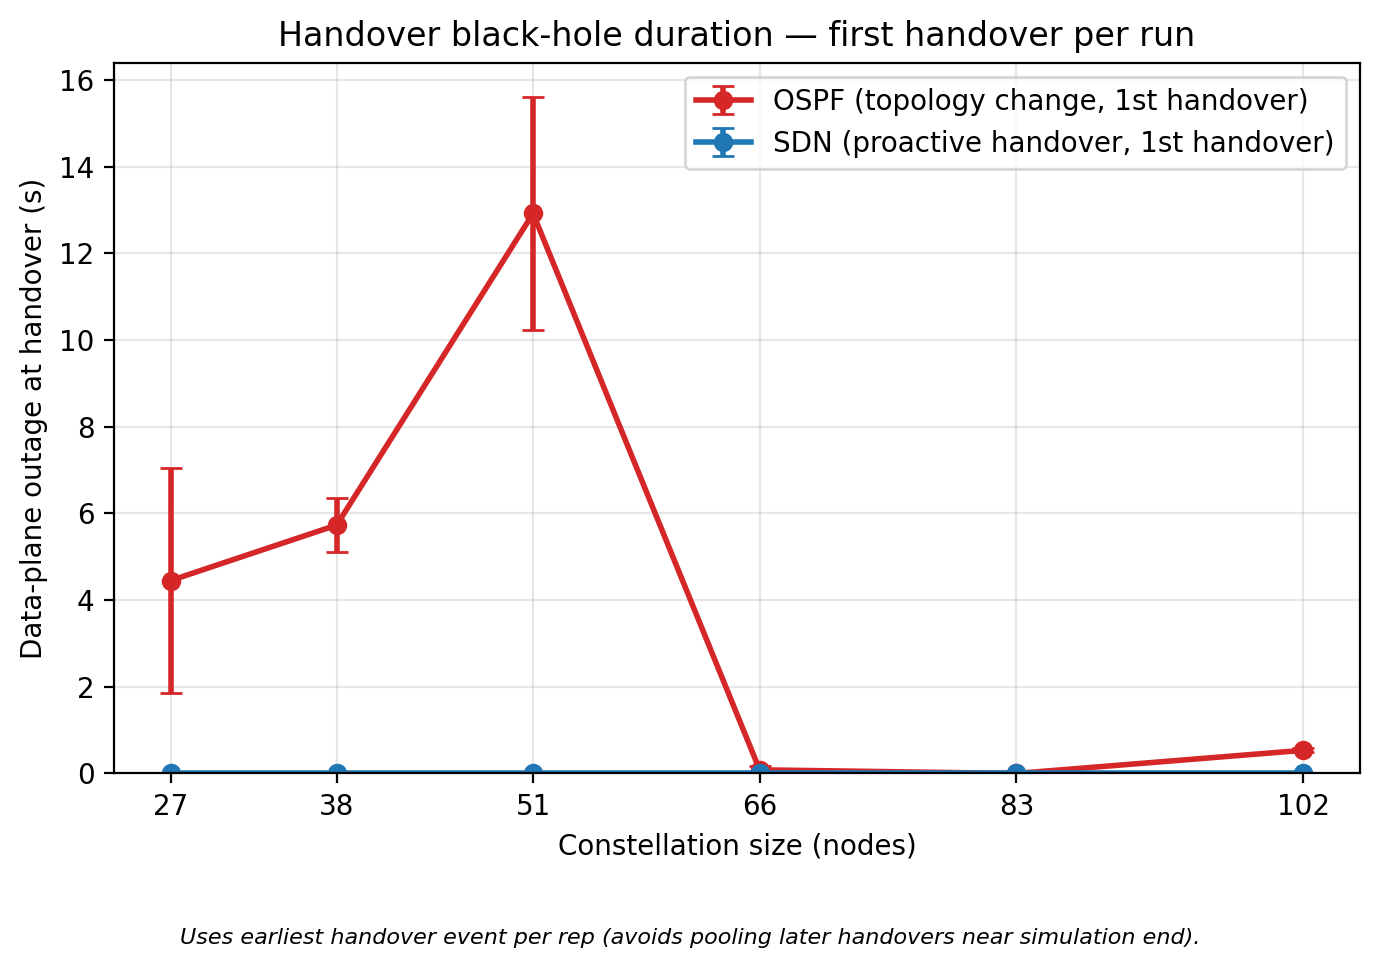
\includegraphics[width=\linewidth]{figures/outage_vs_nodes.png}
  \caption{Mean data-plane outage at the first GSL handover versus constellation
    size ($N$ nodes).
    OSPF (topology-change events) exhibits multi-second black holes;
    OrbitGraph (proactive handover) maintains 0\,s mean outage on every
    grid where the first handover completes inside the emulation window.
    Error bars: standard deviation over ten repetitions.}
  \label{fig:outage-handover}
\end{figure}

Figure~\ref{fig:outage-handover} is the central result of this work.
A continuous ICMP probe inside the source ground-station container
measures sustained loss bursts aligned to control-plane events
(Section~\ref{sec:experiments}); this metric captures downtime that tick-scheduled
pings miss when route installation blocks the emulation loop.

At the first handover, OSPF data-plane outage grows with constellation size and
peaks at ${\sim}13.6$\,s on the $7{\times}7$ grid (51 nodes), with
${\sim}5.7$\,s on $6{\times}6$ (38 nodes) and ${\sim}7.7$\,s on $10{\times}10$
(102 nodes).
These gaps correspond to the interval between GSL teardown and BIRD/OSPF
reconvergence: traffic is forwarded along stale or missing next-hops until
link-state flooding completes~\cite{sidhu:ospf:1993}.

OrbitGraph inverts this picture.
By installing the post-handover FIB after new GSLs are added but \emph{before}
old links are removed (Section~\ref{sec:proactive}), proactive handover yields
0\,ms mean outage on every grid from 27 to 102 nodes, with zero sustained-down
events across all 60 SDN repetitions in the handover cohort.
The data plane stays up even though the container-based install itself takes
seconds (Section~\ref{sec:analysis-control}): make-before-break at the topology
level, not merely at the route-entry level, is what eliminates the black hole.

This is the regime where graph-centric SDN is most effective: GSL handover times
are known from orbital mechanics, the post-handover graph $G_t$ is available in
the delay matrix before the old contact is torn down, and a centralized
controller can commit forwarding for the new graph while both contacts briefly
coexist, something distributed OSPF cannot do without protocol
extensions~\cite{pam:opspf:2019,gregory:satellite-routing:2022}.

\subsection{Reachability and latency across handover phases}
\label{sec:analysis-dataplane}

\begin{figure*}[!t]
  \centering
  \begin{minipage}[t]{0.48\textwidth}
    \centering
    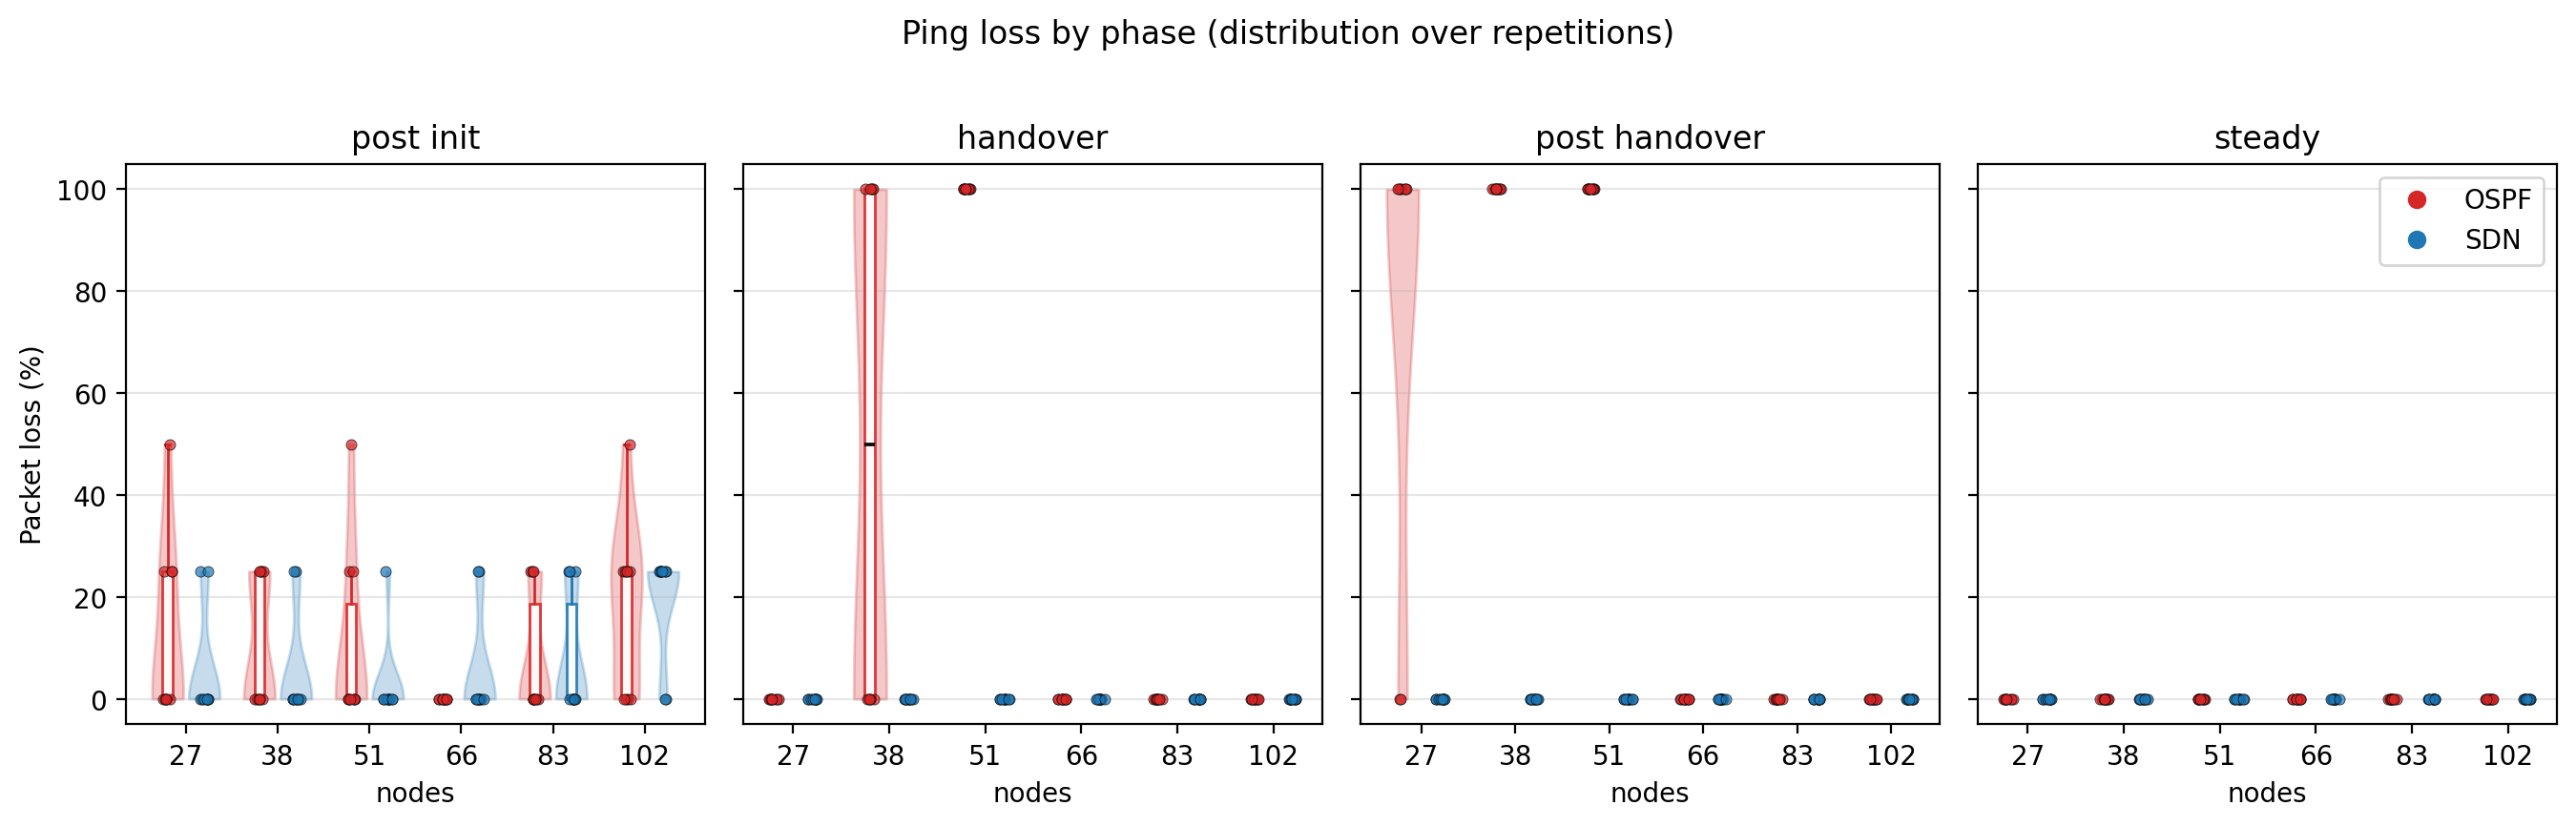
\includegraphics[width=\linewidth]{figures/loss_by_phase.png}\\[-0.5ex]
    {\footnotesize (a) Packet loss by phase}
  \end{minipage}\hfill
  \begin{minipage}[t]{0.48\textwidth}
    \centering
    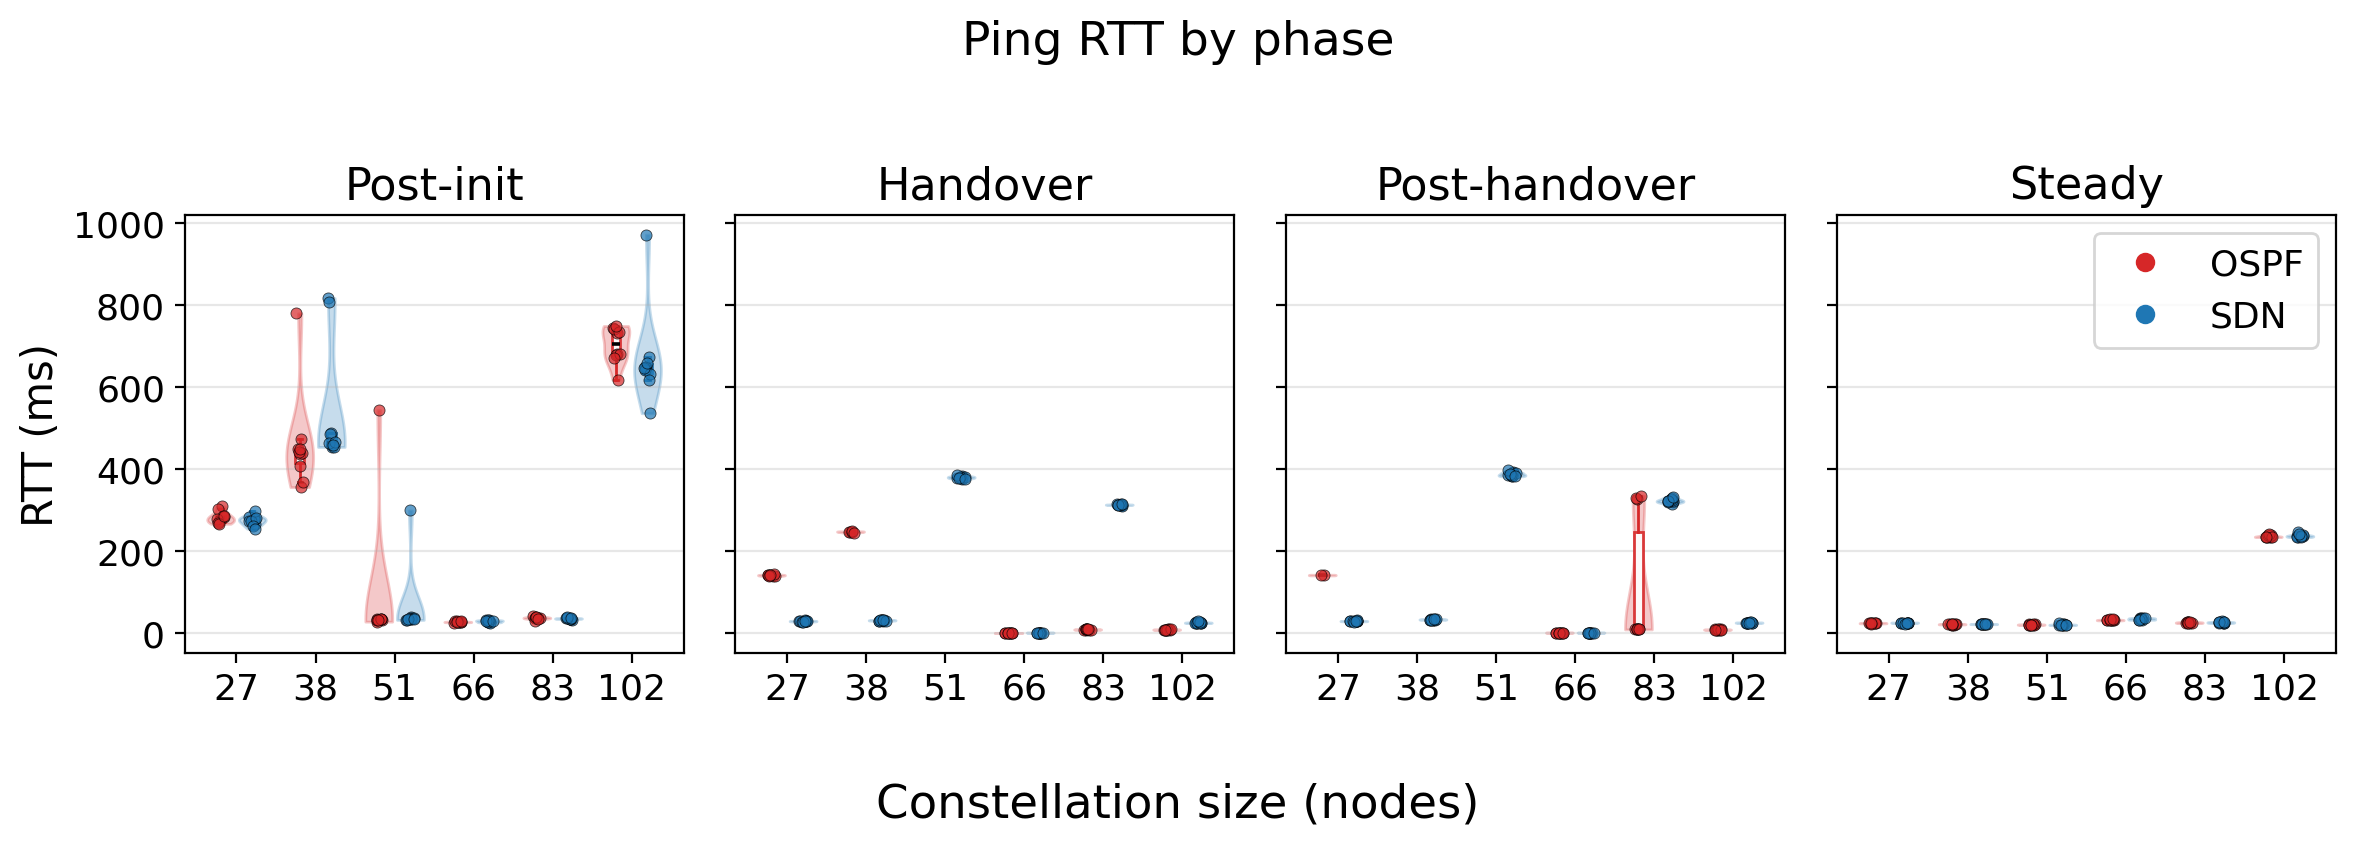
\includegraphics[width=\linewidth]{figures/rtt_by_phase.png}\\[-0.5ex]
    {\footnotesize (b) Mean RTT by phase}
  \end{minipage}
  \caption{End-to-end ground-station ping metrics by handover-relative phase
    (mean~$\pm$~stddev over ten repetitions).
    (a)~Loss; (b)~RTT.
    OrbitGraph holds 0\% loss through handover and post-handover
    on all grid sizes; OSPF loss spikes during reconvergence (e.g., 100\% on
    $7{\times}7$).}
  \label{fig:phase-metrics}
\end{figure*}

Figure~\ref{fig:phase-metrics} complements
Figure~\ref{fig:outage-handover} with scheduled probes at the handover tick,
two seconds later, and near emulation end.

OrbitGraph achieves 0\% mean loss in the handover and post-handover phases on
every grid size.
OSPF loss is highly phase-dependent: on $6{\times}6$ half of handover probes
are lost (50\% mean); on $7{\times}7$ both handover and post-handover phases
reach 100\% loss because the path is black-holed until OSPF settles.
After convergence (steady phase), OSPF recovers to 0\% loss; both modes
eventually forward correctly once the distributed database catches up.

When OrbitGraph keeps the path up, handover-phase RTT reflects the new
shortest path immediately (e.g., ${\sim}380$\,ms on $7{\times}7$ where the
post-handover route is longer).
OSPF either reports no RTT (100\% loss) or misleadingly low values on paths
that are about to break.
At steady state, both modes converge to similar latency (e.g.,
${\sim}236$\,ms on $10{\times}10$), confirming that OrbitGraph does not
degrade steady-state path quality; it changes when the new path becomes
usable, not which shortest path is chosen.

Together, Figures~\ref{fig:outage-handover} and~\ref{fig:phase-metrics}
show that SDN's advantage is not raw steady-state performance but
continuity through predictable topology mutations, the defining challenge
of LEO graph dynamics~\cite{kassing2020exploring,handley:ground-relays:2019}.

\subsection{Control-plane cost and incremental install}
\label{sec:analysis-control}

\begin{figure}[!t]
  \centering
  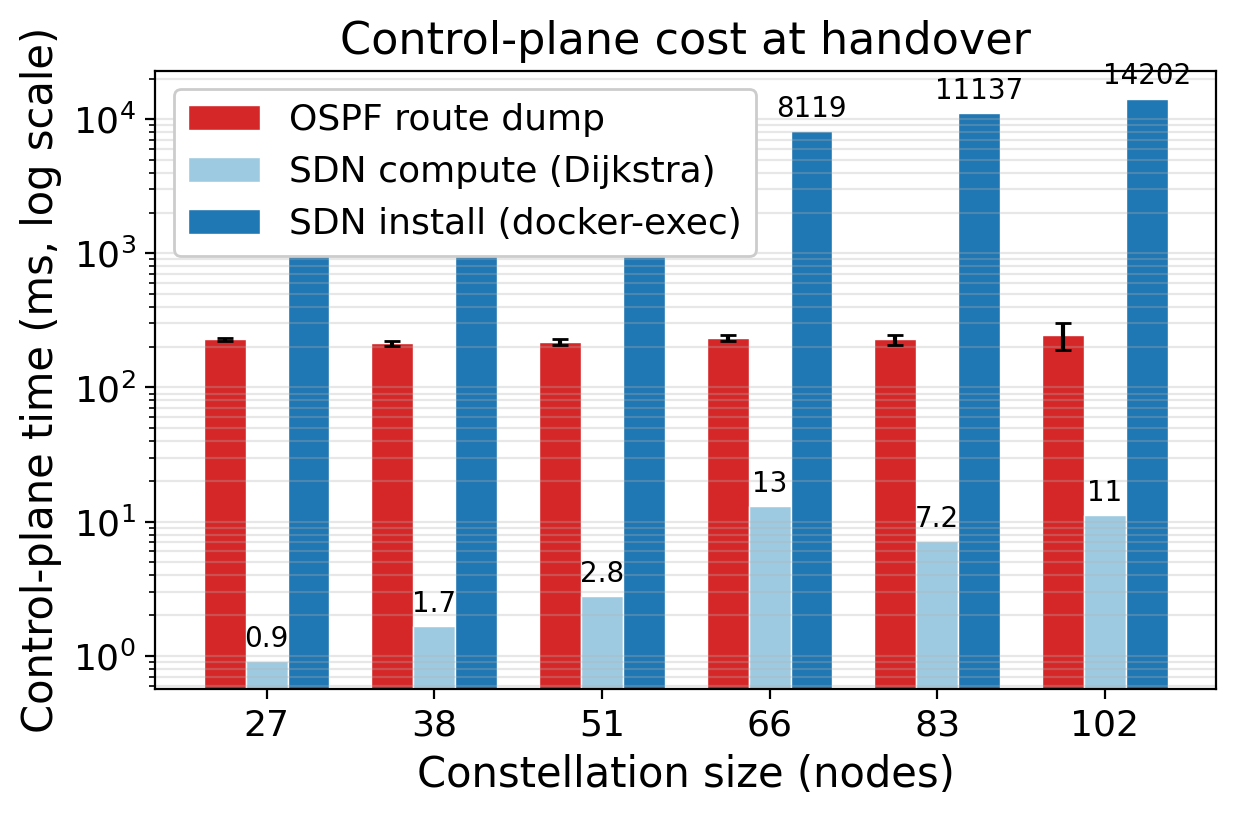
\includegraphics[width=\linewidth]{figures/control_handover.png}
  \caption{Control-plane time at the first handover (log scale).
    OSPF bars show BIRD route-dump collection (${\sim}200$–$230$\,ms).
    OrbitGraph splits algorithmic graph computation (Dijkstra, ${\sim}1$–$12$\,ms)
    from kernel route install (${\sim}3.5$–$14.6$\,s at handover on large grids).}
  \label{fig:control-handover}
\end{figure}

\begin{figure}[!t]
  \centering
  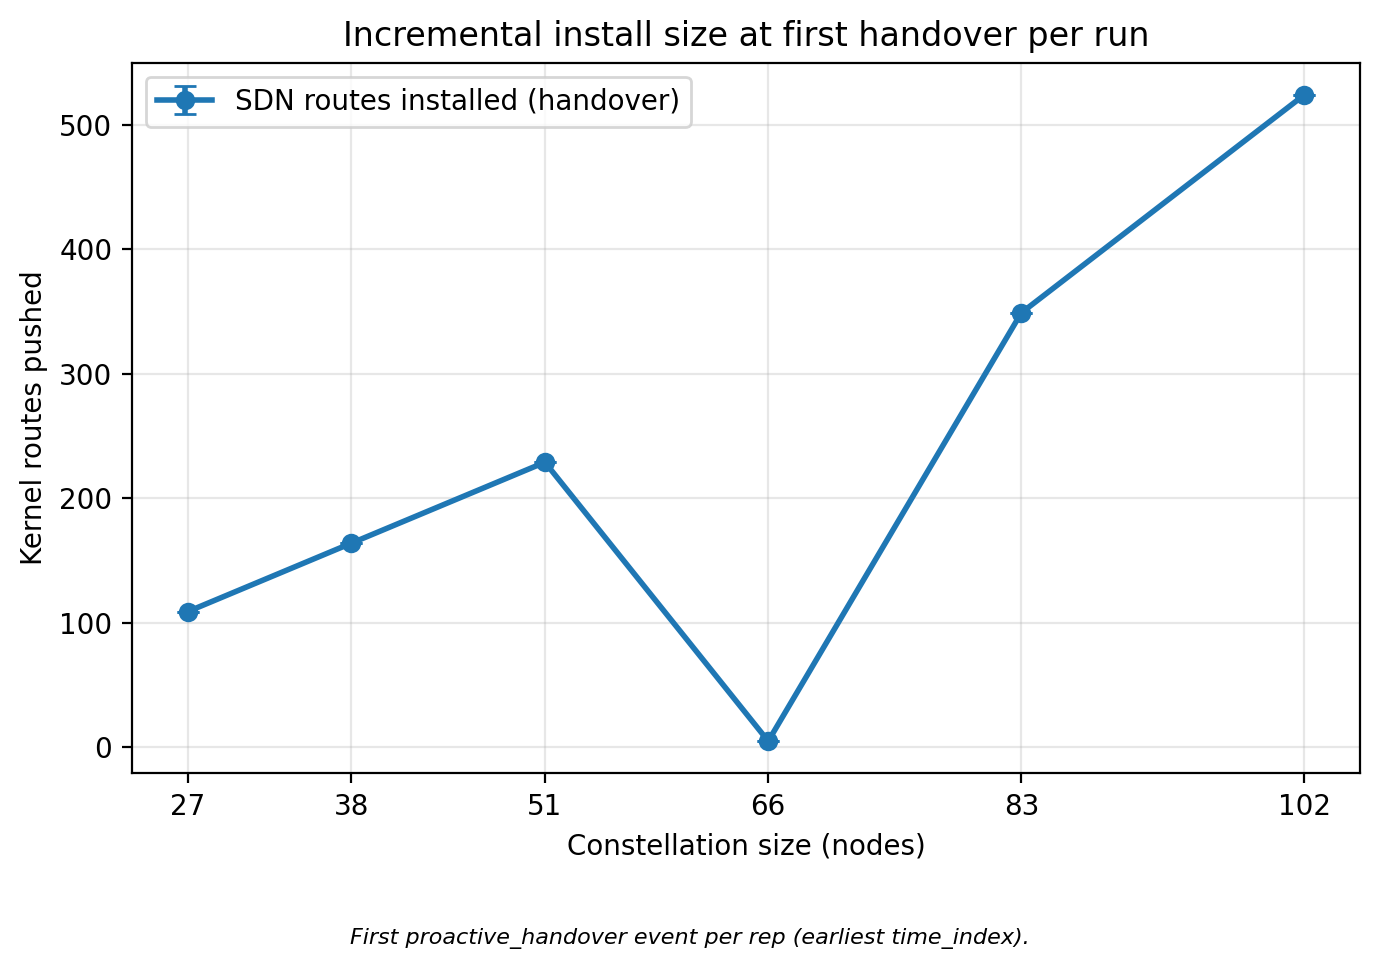
\includegraphics[width=\linewidth]{figures/routes_installed_handover.png}
  \caption{Kernel routes pushed at the first proactive handover (SDN only,
    mean~$\pm$~stddev).
    Incremental install touches hundreds of entries, not the full FIB
    (${\sim}10{,}504$ routes at $10{\times}10$ initialization).}
  \label{fig:routes-handover}
\end{figure}

Figure~\ref{fig:control-handover} separates control-plane algorithm from
dataplane programming.
OrbitGraph's graph recomputation remains in the millisecond range
(${\sim}0.9$–$12.7$\,ms across grids), confirming that shortest-path work on
$G_t$ is not the scalability bottleneck.
What dominates is install time: pushing deltas through per-container
command batches takes ${\sim}3.5$\,s on 27 nodes and
${\sim}14.6$\,s on 102 nodes at the first handover, orders of magnitude more
than OSPF's ${\sim}200$\,ms route observation cost.

This asymmetry is intentional to report honestly.
OSPF's bar measures how long it takes to read routing state after an
event; it does not include the multi-second reconvergence that
Figure~\ref{fig:outage-handover} shows in the data plane.
OrbitGraph's install bar reflects our container southbound harness;
a production SDN plane (gRPC, NETCONF, or on-board agents receiving compressed
deltas) would shrink install time while preserving the same FIB semantics.

Crucially, heavy install does not imply heavy data-plane outage when
updates are ordered proactively: the continuous probe in
Figure~\ref{fig:outage-handover} shows 0\,s black hole even while install runs,
because forwarding entries for the new path are already in place before the old
GSL disappears.

Figure~\ref{fig:routes-handover} explains why install remains tractable.
Incremental deltas (Section~\ref{sec:incremental}) push only changed next-hops:
${\sim}109$ routes at the first handover on $5{\times}5$, rising to
${\sim}576$ on $10{\times}10$, roughly 20$\times$ fewer programming
operations than the ${\sim}10{,}504$ routes required at initialization.
Without incremental install, every handover would replay a full-table push and
amplify the install-time penalty without improving availability.

On delay-only ticks where next-hops are unchanged, OrbitGraph skips the
dataplane entirely (${\sim}1$\,ms compute, zero install).
OSPF incurs no equivalent metric on these ticks, but also cannot proactively
reshape forwarding before a scheduled handover.

\subsection{Resilience under satellite failure}
\label{sec:analysis-damage}

\begin{figure}[!t]
  \centering
  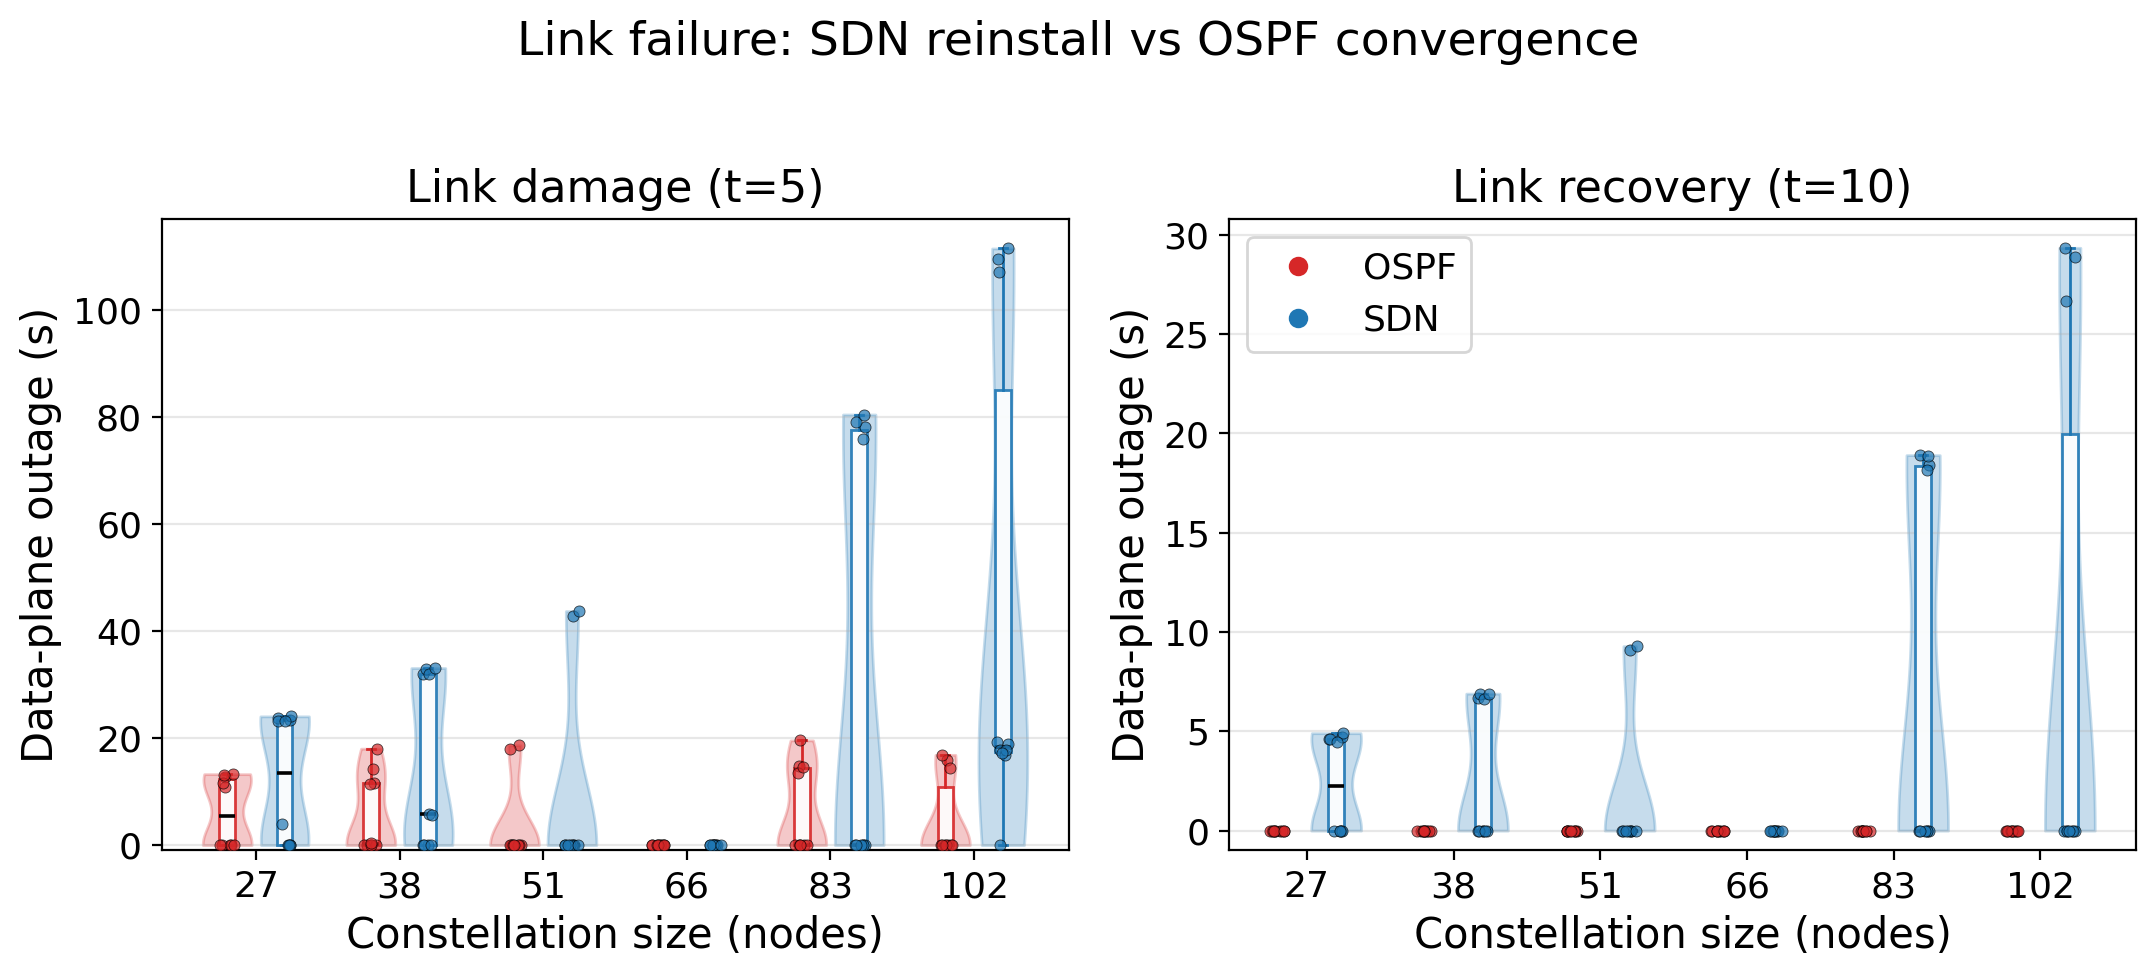
\includegraphics[width=\linewidth]{figures/outage_damage_recovery.png}
  \caption{Data-plane outage after link damage ($t{=}5$) and recovery ($t{=}10$),
    median per repetition.
    OrbitGraph does not outperform OSPF on these events; SDN install
    latency can extend the loss burst relative to distributed reconvergence.}
  \label{fig:outage-damage}
\end{figure}

Figure~\ref{fig:outage-damage} presents a contrasting result, the
regime where OrbitGraph is not the better option in our current implementation.

At $t{=}5$ we disable 30\% of satellites (100\% loss on all interfaces).
Both modes must recompute around a substantially changed $G_t$.
OrbitGraph reacts with a full incremental reinstall (damage recovery),
which blocks the synchronous emulation loop while thousands of routes are pushed.
Median data-plane outage for SDN exceeds OSPF on several grids (e.g.,
${\sim}26$\,s vs.\ ${\sim}2.4$\,s median on 102 nodes in the aggregated cohort).

Three factors explain this gap.
Unlike GSL handover, damage is a reactive event: links fail before the
controller runs, so there is no make-before-break window at the topology level.
Removing 30\% of satellites shifts many next-hops; the install set approaches
a bulk update (${\sim}4{,}700$ routes touched at 102 nodes) rather than the
hundreds seen at handover.
The same container southbound that Figure~\ref{fig:control-handover} shows at
handover applies here without the compensating benefit of proactive link overlap.

After recovery at $t{=}10$, both modes return to low outage on most grids;
neither maintains a decisive advantage.
For unplanned failures, distributed protocols that converge locally, or SDN
with a faster southbound and pipelined delta streaming, remain competitive
with centralized graph recomputation~\cite{gregory:satellite-routing:2022}.

This boundary clarifies OrbitGraph's effective range: scheduled,
orbit-predictable topology changes (GSL handovers, planned ISL reconfiguration)
where global graph knowledge and update ordering translate directly into
zero-outage forwarding continuity.

\subsection{Summary of trade-offs}

Table~\ref{tab:tradeoffs} consolidates the analysis.
OrbitGraph's graph-centric SDN approach delivers its clearest win on end-to-end
availability during contact migration, while trading higher programmatic
control-plane effort (measurable but not user-visible when updates are proactive)
and showing no advantage under bulk failure injection with our current install path.

\begin{table}[!t]
  \centering
  \caption{OrbitGraph vs.\ OSPF: where SDN wins, ties, and lags.}
  \label{tab:tradeoffs}
  \renewcommand{\arraystretch}{1.12}
  \begin{tabular}{@{}p{0.22\linewidth}ccp{0.28\linewidth}@{}}
    \hline
    Scenario & OSPF & OrbitGraph & Comment \\
    \hline
    GSL handover outage      & Multi-second & 0\,ms & Proactive install \\
    Handover/post-HO loss    & Up to 100\% & 0\% & Fig.~\ref{fig:phase-metrics} \\
    Steady-state RTT         & Similar & Similar & Same LeastDelay paths \\
    Dijkstra compute         & n/a & 1–13\,ms & Scales mildly \\
    Route push at handover   & n/a & ${\sim}10^2$–$10^3$ routes & vs.\ ${\sim}10^4$ init \\
    Satellite damage outage  & Lower & Higher & No proactive window \\
    Route-dump / observe     & ${\sim}200$\,ms & n/a & Not reconvergence \\
    \hline
  \end{tabular}
\end{table}

In graph-centric terms, OrbitGraph treats each snapshot $G_t$ as a first-class
object: recomputation is cheap, deltas are small at handover, and update
timing relative to link lifetime is the lever that SDN alone can pull.
Distributed OSPF remains a robust default for unplanned churn and for networks
without a trusted global view; OrbitGraph shows that when the LEO network is
a dynamic graph with known handover schedules, centralized shortest-path control
can keep that graph connected in the data plane through every contact change.

% Future work section for OrbitGraph paper.

\section{Future Work}
\label{sec:future}

Our study demonstrates that graph-centric SDN can eliminate GSL handover black
holes on emulated constellations up to 102 nodes, but several limitations
suggest extensions in experimental methodology, scenario coverage, and
production-scale deployment.

The largest gap between OrbitGraph's algorithmic cost and its observed
control-plane time is kernel route install: pushing routes through per-container
remote execution dominates handover and damage events
(Section~\ref{sec:analysis-control}).
Replacing this harness with a production-style southbound, such as gRPC or
NETCONF to on-board agents with compressed delta messages, would isolate the
true cost of centralized programming from container overhead and likely improve
damage recovery, where install latency currently outweighs global recomputation.
Our synchronous StarryNet loop blocks during route install, inflating outage
measurements for reactive events. Running the controller asynchronously and
timing probes against control-plane timestamps would give a fairer comparison
with distributed protocols, whose reconvergence also overlaps forwarding.
The present campaign uses ICMP probes between two ground stations. Adding
sustained TCP or QUIC flows, multipath traffic matrices, and application-level
quality-of-service metrics would test whether zero handover outage translates
into throughput and goodput gains under realistic load, not only reachability.

Each run already exposes several handover events, which we classify by
ground-station coverage to separate routing behavior from physical connectivity.
Mega-constellations experience continuous contact churn. Emulating multi-hour
windows with dozens of handovers per ground station would reveal whether
incremental baselines stay consistent and whether error accumulation in address
caches or route-key bookkeeping appears over time. Denser constellations would
also close the coverage gaps that a sparse grid exposes at a fixed ground-station
latitude, isolating control-plane behavior from satellite visibility.
Our single autonomous system uses two fixed ground stations and LeastDelay
routing. Extending to multi-AS topologies with BGP peering, or to ground-relay
architectures that offload long-haul traffic to terrestrial
fiber~\cite{handley:ground-relays:2019}, would test OrbitGraph where path
selection crosses administrative boundaries and edge weights are not delay alone.
OrbitGraph proactive handover is complementary to distributed protocols that
exploit ephemeris. A head-to-head study against OPSPF~\cite{pam:opspf:2019} or
segment routing on the same topologies would clarify when centralized install
wins over orbit-predictive link-state flooding, and whether hybrid designs, an
OSPF data plane with SDN-triggered make-before-break, capture most of the
benefit with less operational coupling.
Future scenarios could include capacity-aware weighting beyond delay,
time-varying demand hotspots, partial link degradation such as elevated loss
without total failure, and targeted ISL failures rather than whole-satellite
blackouts.
Section~\ref{sec:analysis-damage} shows OrbitGraph lagging OSPF after
30\% satellite loss because updates are reactive and bulk. Promising directions
include precomputed backup next-hops for known failure domains, staged install
that restores connectivity to ground before refining intra-orbit paths, and soft
damage detection that triggers recomputation before total link loss.

Container emulation allocates one Linux network stack per node. Our workstation
campaign tops out near 102 nodes before memory and CPU become limiting factors,
consistent with observations in the StarryNet literature~\cite{lai2023starrynet}.
Reaching Starlink-class scale (thousands of satellites) requires a tiered
strategy: partition the constellation into orbital planes or regions and run
OrbitGraph per partition with border-route summarization at domain
gateways~\cite{gregory:satellite-routing:2022}; shard containers across hosts
using StarryNet's distributed deployment mode; or combine packet-level emulation
on a representative subgraph with flow-level simulators such as
Hypatia~\cite{kassing2020exploring} or StarPerf~\cite{lai2020starperf} for
full-constellation stress tests, using the same $G_t$ abstraction in both tiers.
Our grids use Walker-style $O{\times}S$ layouts with Starlink-inspired altitude
and inclination but not live two-line element feeds.

Closing the install-time gap, broadening workloads and failure models, and
climbing the scaling ladder through hierarchy and hybrid simulation are the
main levers to move from proof-of-concept to operator-relevant deployment.
The core idea, treating the LEO network as a sequence of graphs, computing
shortest paths centrally, and timing delta installs against known topology
events, remains unchanged; future work fills in the engineering surround
that our current emulation study deliberately simplified.

% Conclusion section for OrbitGraph paper.

\section{Conclusion}
\label{sec:conclusion}

Low Earth orbit mega-constellations are, at their core, dynamic graphs:
vertices are satellites and ground assets, and edges appear and vanish as
orbital geometry evolves. Routing here is not a one-time shortest-path problem
but a continuous sequence of graph snapshots $G_t$ that must reach the
forwarding plane faster than contacts change.
Distributed link-state protocols such as OSPF were designed for topologies that
change sporadically. They discover mutations reactively and reconverge after the
fact, which our measurements show can black-hole traffic for many seconds at
each ground--satellite handover.

Software-defined networking offers a different contract.
By decoupling the control plane from the data plane, OrbitGraph
centralizes graph construction from ephemeris-driven delay
matrices and multi-source Dijkstra while leaving forwarding to the
existing Linux kernel on each node.
The data plane executes simple, fast operations such as longest-prefix match
and local delivery, while the control plane owns global visibility, policy, and
when updates land relative to link lifetime.
That separation is efficient in two senses. Algorithmically, recomputation stays
in the millisecond range even at 102 nodes. Operationally, only changed
next-hops are programmed, ${\sim}10^2$–$10^3$ routes at handover versus
${\sim}10^4$ at initialization, avoiding the cost of re-flooding a full
link-state database to every router on every orbital tick.

The decisive advantage, however, is not raw compute speed but control
over update ordering.
OrbitGraph's proactive handover installs the post-contact FIB while both old and
new ground--satellite links coexist, make-before-break at the topology level.
Distributed OSPF cannot match that behavior without protocol extensions,
because no single router observes the full mutation schedule in advance.
Our container-based evaluation on StarryNet~\cite{lai2023starrynet}, spanning
27 to 102 nodes over ten repetitions, shows 0\,ms data-plane
outage on every coverage-preserving GSL handover against OSPF black holes
reaching ${\sim}15$\,s, 0\% packet loss through handover and post-handover under
OrbitGraph while OSPF loss reaches 100\% on several grids, comparable
steady-state latency, and incremental updates that keep programmatic cost
proportional to handover scope rather than constellation size. Where the
constellation is too sparse to keep a ground station in view, a coverage gap
severs the path for both protocols, delimiting the regime in which control-plane
ordering is decisive.

OrbitGraph demonstrates that graph-centric SDN routing keeps an emulated LEO
network connected through predictable topology changes, the regime where orbital
mechanics already give operators a global view and a contact
schedule~\cite{kassing2020exploring,handley:ground-relays:2019}.
It is not a universal replacement for distributed routing. Under unplanned bulk
failures with our container-based install path, centralized updates can lag
OSPF, and reaching thousands of nodes will require hierarchical control and
faster southbounds.
Within its effective range of scheduled GSL handovers and orbit-predictable
graph snapshots, OrbitGraph shows that treating the constellation as an
explicit, time-indexed graph and programming forwarding from a centralized
controller is a practical path to the sub-second availability that
latency-sensitive space--terrestrial services require.

From a graph-centric computing view, when the network is a graph that changes
on a known timetable, the effective model makes that graph a first-class control
object: recompute on snapshots, push structured deltas, and align commits with
graph edits, rather than forcing each node to infer global state from local
messages.
OrbitGraph is a concrete instantiation of that idea for LEO routing, validated
end-to-end in a real TCP/IP emulation environment with measurable gains in
data-plane availability where it matters most.


% ================ BIBLIOGRAPHY ===================
\bibliographystyle{IEEEtran}
\bibliography{references}

\begin{IEEEbiography}[{
    
\includegraphics[width=0.8\linewidth,clip,keepaspectratio]{figures/pantuza-bio.jpg}}]{Gustavo Pantuza}
    PhD candidate in Computer Science at the Federal University of Minas Gerais. His research areas are networks, distributed systems and observability.
\end{IEEEbiography}

\begin{IEEEbiography}[{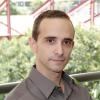
\includegraphics[width=0.8\linewidth,clip,keepaspectratio]{figures/flip-bio.jpg}}]{Luiz Vieira}
is a Professor of Computer Science at the Universidade Federal de Minas Gerais (UFMG). He received his undergraduate and M.S. at the Universidade Federal de Minas Gerais in Belo Horizonte, and Ph. D. degree in Computer Science from the University of California Los Angeles (UCLA). His research interest is in Computer Networking.
\end{IEEEbiography}

\begin{IEEEbiography}[{
    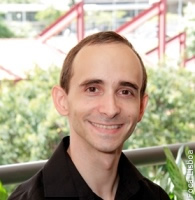
\includegraphics[width=1in,height=1.in,clip]{figures/flop-bio.jpg}}]{Marcos A. M. Vieira} is an Associate Professor of Computer Science at the Universidade Federal de Minas Gerais (UFMG) since 2011. He is awarded a research productivity scholarship level 1 from CNPq. He received his B.Sc. from UFMG in 2002, his M.S. from UFMG in 2004, and his Ph.D. in Computer Science from the University of Southern California (USC) in 2010. Marcos was a Visiting Research Scholar at University of Southern California from 2018 to 2019. His research interests are in Computer Networking and Wireless Networks. He is also a member of IEEE and ACM research communities.
\end{IEEEbiography}


\end{document}


